\section{Punto de Vista de Uso de Tecnología}

El punto de vista de la utilización de la tecnología muestra cómo las aplicaciones son apoyadas por la tecnología de software y hardware: los servicios tecnológicos son suministrados por los dispositivos; el software y las redes del sistema son suministrados a las aplicaciones. Este punto de vista desempeña un papel importante en el análisis del rendimiento y la escalabilidad, ya que relaciona la infraestructura física con el mundo lógico de las aplicaciones. Es muy útil para determinar los requisitos de rendimiento y calidad de la infraestructura en función de las exigencias de las diversas aplicaciones que la utilizan.

\subsection{Modelo de Uso de la Tecnología}
\begin{figure}[h!]
	\centering
	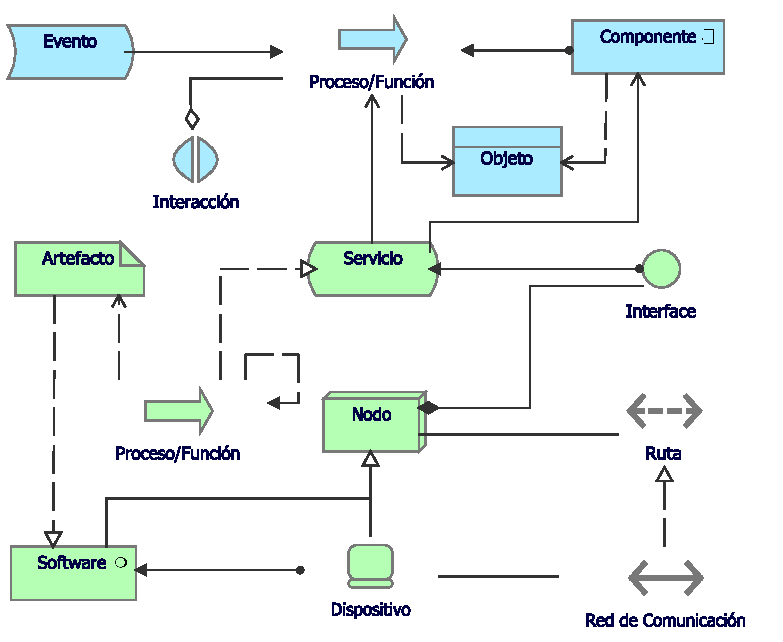
\includegraphics[width=.8\linewidth]{imgs/modelo/UsoTecnologia.pdf}
	\caption{Modelo Implementacion y Despliegue}
\end{figure}

Una función tecnológica describe el comportamiento interno de un nodo; para el usuario de un nodo que realiza una función tecnológica, esta función es invisible. Si su comportamiento es expuesto externamente, esto se hace a través de uno o más servicios tecnológicos. Una función tecnológica se abstrae de la forma en que se implementa. Sólo se especifica el comportamiento necesario. Una función de tecnología puede realizar servicios de tecnología. Los servicios tecnológicos de otras funciones tecnológicas pueden servir a las funciones tecnológicas. Una función tecnológica puede acceder a los objetos tecnológicos. Se puede asignar un nodo a una función tecnológica (lo que significa que el nodo realiza la función tecnológica). El nombre de una función tecnológica debe ser preferentemente un verbo sustantivado.

%\newpage

\subsection{Caso  de  Uso de la Tecnología}
\begin{figure}[h!]
	\centering
	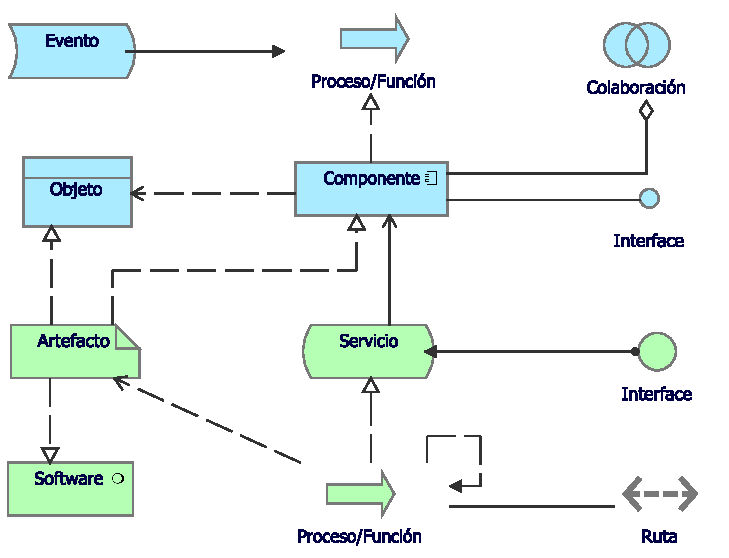
\includegraphics[width=.7\linewidth]{imgs/caso/Implementacion}
	\caption{Caso Implementacion y Despliegue}
\end{figure}
descripcion...